\chapter{Analisis Masalah Dan Rancangan Solusi}

\par Dalam mengadakan kompetisi \textit{competitive programming} diperlukan sebuah sistem \textit{online judge}. Sistem \textit{online judge} memerlukan dua buah komponen utama yaitu \textit{autograder} dan sistem manajemen kompetisi. Sistem manajemen kompetisi memberikan layanan yang berhubungan dengan kompetisi seperti melihat soal, mengirim jawaban, membuat klarifikasi, dan melihat \textit{scoreboard}. Sistem \textit{autograder} berfungsi untuk melakukan penilaian terhadap jawaban yang telah dikirim secara \textit{realtime}. Gambar \ref{fig:architecture-old} menggambarkan arsitektur sistem \textit{online judge} yang saat ini sering digunakan.

\begin{figure}[ht!]
    \centering
    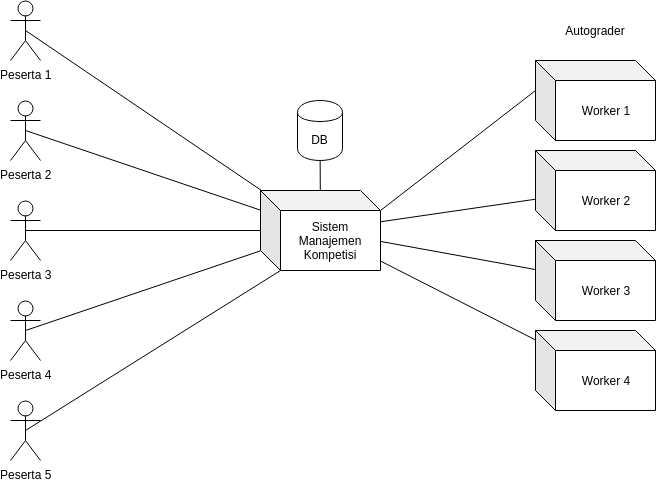
\includegraphics[width=0.7\textwidth]{images/architecture-old}
    \caption{Arsitektur Sistem \textit{Online Judge} Pada Saat Ini}
    \label{fig:architecture-old}
\end{figure}

\section{Sistem \textit{Autograder}} \label{subsec:autograder}

\par Sistem manajemen kompetisi memerlukan \textit{autograder} untuk menilai jawaban peserta kompetisi secara otomatis. Sistem \textit{online judge} yang sering digunakan saat ini menggunakan \textit{autograder} yang dipasang oleh juri pada beberapa komputer yang sudah disediakan oleh juri. Pada tugas akhir ini, diciptakan sistem \textit{autograder} yang dapat berjalan pada komputer peserta. Komputer peserta akan bertindak sebagai \textit{worker} yang menjalankan sistem \textit{autograder}. \textit{Worker} adalah komputer yang digunakan oleh sistem \textit{autograder} untuk melakukan kompilasi dan eksekusi terhadap jawaban peserta. Dalam tugas akhir ini, komputer peserta adalah \textit{worker} dari sistem \textit{autograder}. Terdapat beberapa aspek yang perlu diperhatikan dalam mengembangkan sistem \textit{autograder} seperti pengukuran waktu dan memori, \textit{load balancing}, evaluasi jawaban peserta, dan pengiriman \textit{test-case} ke \textit{worker}. Gambar \ref{fig:architecture-new} menggambarkan arsitektur sistem \textit{online judge} yang dibuat pada tugas akhir ini.

\begin{figure}[ht!]
    \centering
    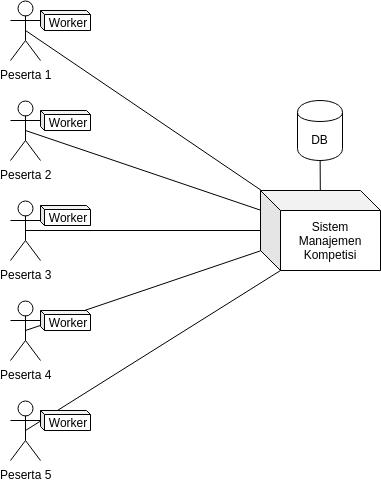
\includegraphics[width=0.5\textwidth]{images/architecture-new}
    \caption{Arsitektur Sistem \textit{Online Judge} Yang Dibuat}
    \label{fig:architecture-new}
\end{figure}

\subsection{Pengukuran Waktu Dan Memori} \label{subsec:time-memory-measure}

\par Komputer peserta memiliki spesifikasi yang berbeda-beda. Perbedaan spesifikasi tersebut menimbulkan beberapa perbedaan ketika sebuah program yang sama dieksekusi. Program yang sama dengan masukan yang sama dapat berjalan dengan waktu dan memori yang berbeda pada komputer yang berbeda. Komputer dengan \textit{clock-speed} yang lebih tinggi akan menjalankan program dengan lebih cepat. Komputer dengan \textit{core} yang lebih banyak juga akan menjalankan program parallel dengan lebih cepat. Selain itu, ukuran \textit{cache} dari komputer juga memengaruhi kecepatan waktu eksekusi. Kebutuhan memori dari suatu program juga ditentukan oleh spesifikasi komputer. Komputer dengan arsitektur 64-bit umumnya memerlukan memori yang lebih besar dibandingkan arsitektur 32-bit. Oleh karena itu, program yang dieksekusi pada komputer yang berbeda akan memerlukan waktu dan memori yang berbeda pula.

\par Penilaian jawaban peserta memerlukan metode pengukuran waktu dan memori yang adil sehingga program peserta yang benar akan dianggap benar oleh setiap \textit{worker}. Begitu juga program peserta yang salah akan dianggap salah oleh setiap \textit{worker}. Pada bab ini, dipaparkan beberapa teknik yang dapat digunakan untuk mengukur waktu eksekusi jawaban peserta.

\subsubsection{Spesifikasi CPU dan Sistem Operasi}

\par Kecepatan eksekusi sebuah program bergantung pada \textit{clock-speed} dan ukuran \textit{cache} dari CPU. Jika suatu proses hanya diberikan satu buah \textit{core} dari CPU, maka jumlah \textit{core} dari CPU dapat dianggap tidak memengaruhi kecepatan eksekusi proses tersebut. Kecepatan eksekusi program dapat diukur berdasarkan spesifikasi CPU dari komputer yang menjalankannya. Program yang dijalankan pada komputer dengan \textit{clock-speed} dan ukuran \textit{cache} yang rendah akan diberikan batasan waktu yang lebih lama. Sedangkan program yang dijalankan pada komputer dengan \textit{clock-speed} dan ukuran \textit{cache} yang lebih tinggi akan diberikan batasan waktu yang lebih singkat. Kebutuhan memori dari program yang dijalankan pada suatu komputer dipengaruhi oleh arsitektur komputer tersebut. Komputer peserta dapat memiliki arsitektur yang berbeda-beda. Komputer dengan arsitektur 64-bit umumnya memerlukan memori yang lebih besar dibandingkan dengan komputer dengan arsitektur 32-bit. Dengan mengetahui arsitektur komputer, kebutuhan memori dari suatu program dapat diperkirakan.

\par Pada penilaian jawaban peserta, diperlukan pengukuran waktu dan memori yang sangat akurat. Pengukuran waktu atau memori yang tidak akurat akan menimbulkan ketidakadilan dalam melakukan penilaian jawabab peserta. Dengan hanya memerhatikan spesifikasi dari CPU dan sistem operasi pada komputer peserta, pengukuran waktu dan memori yang akurat sulit dilakukan. Program yang berjalan pada sistem operasi 64-bit tidak selalu memerlukan memori dua kali dari program yang berjalan pada sistem operasi 32-bit. Kebutuhan memori bergantung pada isi dari program yang dijalankan dan beberapa faktor lain. Kecepatan eksekusi dari suatu program pun bergantung dari beberapa faktor lain sehingga pengukuran waktu dengan cara ini sulit untuk dilakukan.

\subsubsection{CPU \textit{Benchmarking}}

\par \textit{Benchmarking} dapat dilakukan untuk mengukur kinerja CPU dengan menggunakan sebuah program \textit{test}. Program \textit{test} dapat dijalankan pada CPU untuk mengukur waktu eksekusinya. Program \textit{test} yang dijalankan pada komputer pengguna akan dicatat jumlah instruksi dan waktunya. Jumlah instruksi dan waktu yang dibutuhkan untuk menjalankan program \textit{test} dapat digunakan untuk mengukur kinerja CPU. Batas waktu dari jawaban peserta kemudian ditentukan berdasarkan hasil eksekusi program \textit{test} tersebut.

\par \textit{Benchmarking} pada komputer peserta memiliki celah keamanan. Peserta bisa saja menjalankan program yang berat ketika proses \textit{benchmarking} dilakukan. Hal ini akan menyebabkan waktu eksekusi menjadi lambat dan dapat meningkatkan batasan waktu dari jawaban peserta.

\par Selain adanya celah keamanan, terdapat kesulitan lain yang ditemukan ketika melakukan \textit{benchmarking} yaitu pembuatan program \textit{test}. Program \textit{test} perlu dibuat sedemikian rupa sehingga dapat memberikan pengukuran waktu dan memori yang akurat. Untuk mengukur waktu eksekusi dan penggunaan memori dari program peserta dengan kompleksitas yang berbeda, diperlukan program \textit{test} yang berbeda. Hal ini mengakibatkan perlunya membuat program \textit{test} untuk setiap jenis soal yang ada pada kompetisi \textit{competitive programming}. Pembuatan program \textit{test} ini kemudian memberatkan juri karena juri perlu memikirkan program \textit{test} yang cocok sehingga dapat memberikan pengukuran waktu dan memori yang akurat.

\subsubsection{\textit{Benchmarking} Dengan Solusi Juri} \label{subsec:time-memory-measure-compare-with-jury}

\par Teknik \textit{benchmarking} sebenarnya efektif digunakan oleh \textit{autograder} untuk melakukan pengukuran waktu. Meskipun begitu, teknik \textit{benchmarking} tidak efisien dan memiliki celah keamanan jika digunakan. Juri perlu membuat sebuah program \textit{test} untuk setiap soal yang diberikan kepada peserta. Hal ini memberatkan pekerjaan juri sehingga dinilai tidak efisien. Selain itu, peserta dapat menjalankan proses yang berat pada komputernya sehingga memengaruhi keakuratan teknik \textit{benchmarking}.

\par Terdapat teknik yang dapat digunakan untuk meningkatkan efisiensi teknik \textit{benchmarking}. Teknik \textit{benchmarking} dapat menjadi lebih efisien dengan menghindari pembuatan program \textit{test} dari setiap soal pada kompetisi \textit{competitive programming}. Setiap soal dari kompetisi \textit{competitive programming} memiliki solusi yang telah dibuat juri. Solusi dari juri tersebut dapat digunakan sebagai program \textit{test}. Solusi \textit{juri} memiliki kompleksitas yang sesuai dengan soal yang telah dibuat oleh juri sehingga dapat menjadi program \textit{test} yang dapat digunakan untuk mengukur waktu eksekusi dan penggunaan memori dari program peserta secara akurat. Dengan menggunakan solusi juri sebagai program \textit{test}, juri tidak perlu membuat program \textit{test} khusus sehingga proses \textit{benchmarking} dapat menjadi lebih efisien.

\par Selain masalah efisiensi, teknik \textit{benchmarking} juga memiliki permasalahan lain yaitu bagaimana menghindari kecurangan peserta. Peserta bisa saja menjalankan proses yang berat pada komputernya sehingga mengganggu keakuratan proses \textit{benchmarking}. Hal ini menyebabkan sistem \textit{autograder} menganggap bahwa komputer peserta merupakan komputer yang lambat dan mengakibatkan jawaban peserta yang lambat bisa jadi dianggap jawaban yang benar.

\par Terdapat teknik yang dapat digunakan untuk menghindari kecurangan peserta pada paragraf sebelumnya. Pengukuran waktu yang dilakukan pada saat benchmarking dapat dilakukan dengan hanya memperhitungkan \textit{CPU Time}. \textit{CPU Time} merupakan waktu dimana proses sedang dijadwalkan untuk dieksekusi oleh \textit{CPU}. Ketika peserta menjalankan banyak proses yang berat, maka \textit{CPU} akan dijadwalkan untuk mengeksekusi proses yang terkait dengan \textit{autograder} secara lebih jarang. Hal ini dikarenakan sistem operasi membagikan \textit{CPU} secara adil untuk seluruh proses yang ada. Dengan cara ini, waktu yang dijadwalkan untuk proses lain tidak akan dihitung dalam \textit{benchmarking}.

\par Sistem operasi berbasis Linux menyediakan fitur \textit{cgroup} yang dapat digunakan untuk melakukan pengukuran \textit{CPU Time} dari suatu proses. Dengan menggunakan \textit{cgroup}, \textit{resource} yang digunakan oleh proses dapat dipantau. \textit{Cgroup} memungkinkan suatu proses untuk memantau penggunaan CPU dan memori dari proses lain. 

\begin{figure}[ht!]
    \centering
    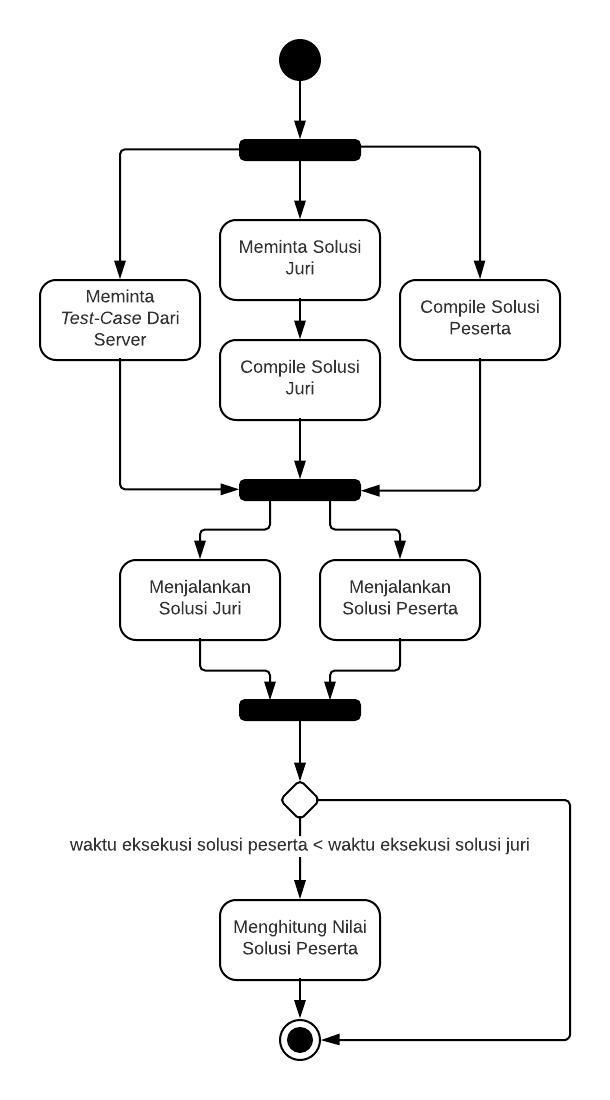
\includegraphics[width=0.5\textwidth]{images/cpu-time-counting}
    \caption{Diagram Aktivitas Penilaian Solusi Peserta}
    \label{fig:cpu-time-counting}
\end{figure}

\par \textit{Autograder} perlu menentukan apakah solusi peserta masih berada pada batas waktu yang diinginkan oleh juri. Hal tersebut dapat dicapai dengan membandingkan waktu eksekusi solusi peserta dengan waktu eksekusi solusi juri. Jika waktu eksekusi solusi peserta masih lebih cepat dari waktu eksekusi solusi juri, maka solusi peserta akan dianggap memenuhi batas waktu.

\par Meskipun solusi juri dan solusi peserta dieksekusi pada komputer yang sama. Waktu eksekusi kedua program tersebut dapat sedikit berbeda karena adanya perbedaan implementasi antara solusi peserta dan juri. Solusi peserta bisa saja lebih lambat atau lebih cepat dibandingkan dengan solusi juri. Untuk mengatasi perbedaan waktu ini, sebuah faktor toleransi dapat diterapkan pada sistem \textit{autograder}. Solusi peserta dapat diterima jika waktu eksekusinya masih berada pada batas toleransi dari solusi juri. Secara matematis, solusi peserta akan diterima jika memenuhi persamaan berikut $ T_{peserta} < (1 + \gamma) \times T_{juri}$, dengan $\gamma$ adalah nilai dari faktor toleransi.

\par Dengan membandingkan penggunaan CPU dan memori dari solusi peserta dengan solusi juri, perhitungan waktu dan memori yang akurat dapat dilakukan. Meskipun peserta menjalankan program yang berat pada saat penilaian dilakukan, perbandingan waktu eksekusi dari program solusi juri dengan program solusi peserta akan tetap sama. Oleh karena itu, teknik ini digunakan untuk melakukan pengukuran waktu dan memori dalam menyelesaikan tugas akhir ini. Gambar \ref{fig:cpu-time-counting} menjelaskan proses penilaian jawaban peserta dengan membandingkan dengan program solusi juri. 

\lstinputlisting[caption={Contoh Program yang \textit{IO bound}},label={lst:busysleeping},language=C,style=CStyle]{listings/busy-sleep.c}

\par Dengan hanya menghitung \textit{CPU Time} dari proses, terdapat masalah lain yang muncul. Peserta bisa saja mengirimkan jawaban berupa program yang bersifat \textit{IO bound}. Program yang bersifat \textit{IO bound} tidak menggunakan banyak \textit{CPU Time}. Kode \ref{lst:busysleeping} merupakan contoh program yang bersifat \textit{IO bound}. Program tersebut tidak menggunakan banyak \textit{CPU Time} karena hanya melakukan \textit{sleep}. Pada saat \textit{sleep}, proses yang berjalan tidak akan dijadwalkan untuk dieksekusi oleh \textit{CPU}. Hal tersebut menyebabkan proses dapat berjalan dengan sangat lama akan tetapi \textit{CPU Time}-nya bernilai hampir nol. Program tersebut akan mengakibatkan \textit{autograder} tidak pernah selesai melakukan pengukuran waktu karena \textit{CPU Time}-nya sangat kecil dan proses tidak pernah selesai untuk dijalankan.

\par Untuk mengatasi proses yang bersifat \textit{IO bound}, waktu eksekusi dapat dibatasi oleh \textit{wall-clock time}. \textit{Wall-clock} merupakan waktu sebenarnya dimana proses berada berada dalam sistem operasi komputer. Proses yang berjalan ketika melakukan \textit{benchmarking} dapat dibatasi \textit{Wall-clock time}-nya. Batas \textit{wall-clock time} dapat diatur sedemikian rupa sehingga dapat dipastikan bahwa solusi peserta yang melewati batas ini dipastikan tidak lolos. Salah satu contoh batas \textit{wall-clock time} adalah satu detik ditambah lamanya \textit{CPU time} dari proses eksekusi solusi juri.

\par Penentuan batas \textit{wall-clock time} sulit dilakukan pada komputer dengan spesifikasi yang berbeda-beda. Komputer yang berbeda mungkin memiliki kecepatan \textit{IO} yang berbeda. Hal ini mengakibatkan juri perlu memerhatikan spesifikasi setiap komputer peserta untuk mengatur nilai \textit{wall-clock time} yang tepat. Selain itu, setiap proses pada sistem operasi yang berbasis Linux memiliki prioritas yang dapat diatur. Peserta bisa saja menjadikan sistem \textit{autograder} memiliki prioritas rendah sehingga proses yang melakukan pengukuran waktu jarang dijadwalkan oleh sistem operasi. Hal tersebut mengakibatkan berkurangnya keakuratan proses \textit{benchmarking}.

\par Untuk mengatasi permasalahan pada paragraf di atas, kecepatan \textit{IO} dari setiap komputer peserta yang digunakan untuk pengukuran waktu dapat dibatasi sehingga seluruh komputer peserta memiliki kecepatan \textit{IO} yang sama. Selain itu, proses \textit{autograder} dapat diatur untuk memiliki prioritas yang tinggi sehingga lebih sering dijadwalkan oleh sistem operasi. Pada tugas akhir ini solusi tersebut tidak digunakan karena masih perlu adanya penelitian lebih lanjut. Pada tugas akhir ini, ketika pengukuran waktu sudah melebihi batas \textit{wall-clock time}, \textit{autograder} akan memberikan \textit{verdict} \textit{Internal Error} yang menandakan proses penilaian gagal. Penilaian yang gagal tidak akan dihitung dan akan dijadwalkan untuk dikerjakan oleh komputer peserta lain. 

\subsection{\textit{Load Balancing}}

\begin{figure}[ht!]
    \centering
    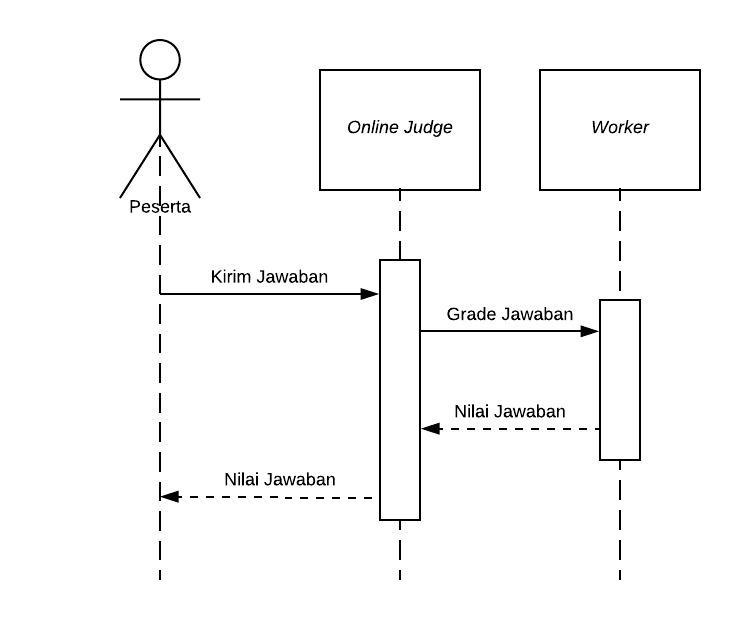
\includegraphics[width=0.75\textwidth]{images/load-balancing-push}
    \caption{\textit{Push-Based Load Balancer}}
    \label{fig:load-balancing-push}
\end{figure}

\par Dalam membangun sistem \textit{autograder}, diperlukan pembagian kerja kepada \textit{worker-worker} yang ada. \textit{Worker} yang dimaksud adalah komputer yang bekerja melakukan penilaian jawaban peserta. Dalam tugas akhir ini, \textit{worker} merupakan komputer peserta. Karena spesifikasi komputer tiap \textit{worker} berbeda-beda, diperlukan teknik pembagian kerja yang adil kepada seluruh seluruh \textit{worker}. Selain itu, aspek keamanan juga perlu diperhatikan karena jawaban peserta akan dikirimkan ke \textit{worker} lain. Terdapat beberapa pendekatan pembagian kerja yang dapat digunakan, yaitu: \textit{push-based}, \textit{pull-based}, dan \textit{self-grading}.

\par Pada pendekatan \textit{push-based}, sistem \textit{autograder} memerlukan sebuah \textit{master} yang akan membagikan pekerjaan ke seluruh \textit{worker}. \textit{Master} akan menentukan \textit{worker} mana yang akan diberikan suatu pekerjaan. Dengan menggunakan metode ini, \textit{master} perlu mengetahui informasi \textit{resource} dari seluruh \textit{worker} yang ada. Setiap \textit{worker} perlu mengirimkan informasi \textit{resource}-nya kepada \textit{master}. Metode ini cukup sulit untuk dilakukan karena perlunya mengimplementasikan algoritma \textit{load balancing} pada \textit{master}. Gambar \ref{fig:load-balancing-push} menggambarkan alur pembagian kerja dengan metode \textit{push-based}.

\begin{figure}[ht!]
    \centering
    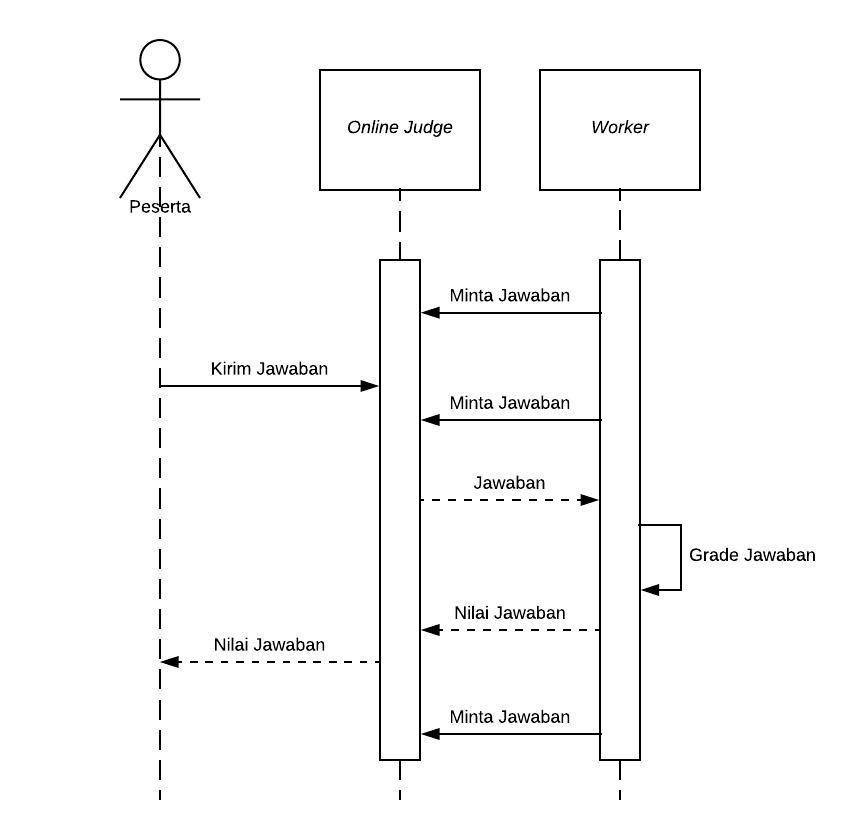
\includegraphics[width=0.75\textwidth]{images/load-balancing-pull}
    \caption{\textit{Pull-Based Load Balancer}}
    \label{fig:load-balancing-pull}
\end{figure}

\par Pada pendekatan \textit{pull-based}, diperlukan juga sebuah \textit{master} yang akan menyimpan seluruh pekerjaan yang perlu diselesaikan. Pendekatan \textit{pull-based} berbeda dengan pendekatan \textit{push-based} dimana \textit{master} lah yang memberikan pekerjaan kepada \textit{worker}. Pada pendekatan \textit{pull-based}, \textit{worker} yang sedang tersedia akan meminta pekerjaan kepada \textit{master}. Dengan pendekatan ini, pembagian pekerjaan akan menjadi rata dengan sendirinya. Metode ini lebih mudah untuk diimplementasikan dibanding dengan metode \textit{push-bashed} karena tidak perlu membuat algoritma \textit{load balancing} yang spesifik pada \textit{master}. Gambar \ref{fig:load-balancing-pull} menggambarkan alur pembagian kerja dengan metode \textit{pull-based}.

\par Selain pendekatan \textit{push-based} dan \textit{pull-based}, terdapat pendekatan lain yang lebih sederhana yaitu \textit{self-grading}. Pada \textit{self-grading}, peserta akan menilai jawabannya sendiri. Dengan menggunakan pendekatan ini, tidak diperlukan adanya \textit{master}. Meskipun begitu, pendekatan \textit{self-grading} memiliki celah keamanan karena peserta mengetahui jawaban siapa yang dinilai pada komputernya. Hal ini memungkinkan peserta untuk melakukan serangan-serangan yang mengakibatkan jawaban yang dinilai pada komputernya selalu dianggap benar.

\par Pendekatan \textit{pull-based} lebih adil dan lebih mudah diimplementasikan dibandingkan dengan pendekatan \textit{push-based}. Pendekatan \textit{pull-based} lebih aman dibandingkan dengan pendekatan \textit{self-grading} karena identitas jawaban yang dinilai pada \textit{worker} lebih rahasia. Oleh karena itu, pendekatan \textit{pull-based load balancing} digunakan pada tugas akhir ini karena lebih adil dan lebih aman dibandingkan dengan dua pendekatan lainnya.

\par Untuk meningkatkan keamanan, jawaban peserta dapat dinilai pada lebih dari satu buah \textit{worker}. Jawaban peserta dinilai benar jika mayoritas dari \textit{worker} yang menilai jawaban peserta tersebut menyatakan bahwa jawaban tersebut adalah benar. Dengan menilai jawaban peserta di banyak \textit{worker}, risiko yang timbul sebab adanya kecurangan yang dilakukan peserta dapat berkurang. Pada tugas akhir ini, \textit{load balancing} dilakukan dengan pendekatan \textit{pull-based} dan dengan melakukan penilaian jawaban peserta pada lebih dari satu buah \textit{worker}.

\subsection{Evaluasi Jawaban Menggunakan Sandbox}

\par Dalam melakukan penilaian terhadap jawaban peserta, diperlukan adanya proses kompilasi dan eksekusi terhadap program yang dikirimkan peserta. Proses kompilasi dan eksekusi ini akan dijalankan pada \textit{worker}. Proses ini dapat membahayakan lingkungan \textit{worker} jika peserta mengirimkan kode program yang berbahaya. Untuk menghindari kerusakan pada \textit{worker}, proses ini perlu diisolasi sehingga tidak berpengaruh pada lingkungan \textit{worker}. Teknik untuk mengisolasi proses eksekusi program ini dinamakan \textit{sandboxing}. Terdapat beberapa teknik \textit{sandboxing} yang dapat digunakan seperti \textit{virtual machine} dan \textit{containerization}.

\subsubsection{Menggunakan \textit{Virtual Machine}}

\par \textit{Virtual machine} memberikan isolasi kepada program pada tingkat \textit{hardware}. Komputer yang ada pada saat ini memiliki \textit{hypervisor} yang dapat digunakan untuk menyimulasikan \textit{hardware} dari komputer. Dengan menggunakan \textit{virtual machine}, komputer dapat menjalankan sistem operasi virtual di atas sistem operasi yang sedang berjalan. \textit{Virtual machine} memberikan layanan isolasi yang sangat aman.

\par Meskipun keamanan \textit{virtual machine} sangat tinggi, akan tetapi banyak \textit{overhead} yang ditimbulkan. Untuk menyalakan \textit{virtual machine}, membutuhkan waktu yang lama dan memori yang cukup besar. Selain itu, diperlukan adanya sistem operasi baru yang berjalan di atas \textit{virtual machine} yang dibuat. Hal ini menyebabkan proses penilaian jawaban peserta menjadi lambat dan membutuhkan sangat banyak memori.

\subsubsection{Menggunakan \textit{Container}}

\par \textit{Container} merupakan suatu teknik untuk mengisolasi proses pada tingkat \textit{software}. Dengan menggunakan \textit{container}, proses yang berjalan pada sistem operasi berbasis Linux dapat dibatasi \textit{resource}-nya. Penggunaan memori dan CPU dari suatu proses dapat dibatasi sehingga tidak membebani komputer peserta. Selain itu, Linux memiliki fitur yang memungkinkan pengguna mengisolasi suatu proses sehingga proses tersebut tidak dapat mengatahui informasi rahasia yang ada pada komputer peserta. \textit{Container} dapat dibuat dengan memanfaatkan fitur dari sistem operasi berbasis Linux yaitu: \textit{chroot}, \textit{namespace}, \textit{rlimit} dan \textit{cgroup}. Pada tugas akhir ini, \textit{container} digunakan untuk melakukan isolasi pada proses yang berjalan pada komputer peserta. Teknik ini dipilih karena memberikan isolasi yang cukup, dan tidak menimbulkan \textit{overhead} yang sangat besar seperti teknik isolasi dengan \textit{virtual machine}.

\par \textit{Chroot} memungkinkan proses pada sistem operasi berbasis Linux untuk memiliki \textit{filesystem} sendiri. Hal ini dapat dilakukan dengan mengganti \textit{root} dari proses ke \textit{directory} tertentu. Dengan mengganti \textit{root}, maka proses tidak dapat mengakses \textit{file} yang berada di luar \textit{directory root}. \textit{Chroot} dapat dilakukan dengan melakukan pemanggilan \textit{system call chroot}. \textit{System call chroot} hanya dapat dilakukan oleh proses yang memiliki akses \textit{root} atau memiliki \textit{capability} \textit{CAP\_SYS\_CHROOT}. Pada tugas akhir ini, program \textit{autograder} diberikan akses \textit{root} sehingga dapat melakukan pemanggilan \textit{system call chroot}.

\par \textit{Namespace} merupakan fitur dari Linux yang memungkinkan pengisolasian suatu proses sehingga tidak mengetahui informasi lain di luar \textit{namespace}-nya. Setiap proses pada Linux memiliki \textit{namespace}. Proses yang berada pada \textit{namespace} tidak akan mengetahui informasi dari \textit{namespace} lain. Hal ini memungkinkan suatu proses untuk diisolasi sehingga tidak mengatahui adanya proses lain, \textit{user} lain, ataupun \textit{network interface} lain. Dengan menggunakan \textit{namespace}, keamanan dari lingkungan \textit{worker} dapat dijaga karena jawaban peserta tidak mengetahui informasi mengenai komputer peserta. Pada tugas akhir ini, proses evaluasi jawaban peserta dilakukan di dalam \textit{namespace} yang terpisah dari \textit{namespace} pengguna.

\par Setiap proses pada sistem operasi berbasis Linux memiliki batas \textit{resource} yang dapat digunakan. Batas tersebut dapat diatur dengan melakukan pemanggilan \textit{system call setrlimit}. Proses yang menggunakan \textit{resource} melebihi batas akan dihentikan oleh sistem operasi. Pada tugas akhir ini, \textit{system call setrlimit} digunakan untuk membatasi jumlah proses yang dapat diciptakan, jumlah \textit{open file descriptor} yang dapat dimiliki, dan ukuran file yang dapat diciptakan oleh program peserta.

\par \textit{Cgroup} merupakan fitur dari sistem operasi berbasis Linux yang dapat digunakan untuk membatasi penggunaan \textit{resource} suatu proses. Selain itu, \textit{cgroup} juga dapat digunakan untuk memantau penggunaan \textit{resource} dari proses tersebut. Pada tugas akhir ini, \textit{cgroup} digunakan untuk mengukur penggunaan CPU dan memori dari proses yang berjalan dan menghentikan proses yang menggunakan \textit{resource} secara berlebihan.

\subsection{Kompilasi Program}

\par Penilaian terhadap jawaban peserta memerlukan adanya tahap kompilasi agar program dapat dijalankan. Keamanan dari proses kompilasi tentunya juga perlu dijaga. Keamanan dari proses kompilasi dapat dicapai dengan menggunakan \textit{sandbox} seperti yang sudah dijelaskan pada subbab sebelumnya.

\par Salah satu aspek yang perlu diperhatikan dalam melakukan kompilasi adalah pengadaan \textit{compiler}. \textit{Compiler} merupakan program yang digunakan untuk melakukan kompilasi kode sumber menjadi program yang dapat dijalankan pada sistem operasi. Komputer peserta tentunya perlu memiliki \textit{compiler} untuk melakukan kompilasi. Untuk menjaga keadilan, seluruh \textit{compiler} yang ada pada komputer peserta perlu memiliki versi yang sama. \textit{Compiler} dengan versi yang berbeda dapat menghasilkan program dengan kemampuan yang berbeda. Terkadang \textit{compiler} dengan versi yang lebih baru dapat memberikan optimisasi pada program sehingga berjalan dengan lebih cepat. Perbedaan versi \textit{compiler} pada komputer peserta akan memberikan ketidakadilan dalam proses penilaian.

\par Masalah pada paragraf sebelumnya diatasi dengan melengkapi \textit{autograder} dengan \textit{compiler}. Karena ukuran \textit{compiler} umumnya cukup besar, maka \textit{compiler} di-\textit{compress} ketika didistribusikan ke komputer peserta. Setiap sistem \textit{autograder} dijalankan, \textit{compiler} akan di-\textit{extract} sehingga siap digunakan.

\subsection{Pengiriman \textit{Test-Case} Ke \textit{Worker}} \label{subsec:sending-test-case-to-worker}

\par Dalam melakukan penilaian jawaban peserta perlu adanya pengiriman \textit{test-case} dari \textit{server} ke \textit{worker}. \textit{Test-case} merupakan informasi yang digunakan untuk menentukan kebenaran jawaban peserta sehingga informasi ini bersifat rahasia dan tidak boleh diketahui oleh peserta maupun orang lain di luar kompetisi. \textit{Test-case} digunakan sebagai masukan pada saat menjalankan program solusi peserta dan juri. Kebenaran dari solusi peserta dinilai dari keluaran yang dihasilkan. Salah satu cara untuk menilai kebenaran program peserta tersebut adalah dengan membandingkan keluaran program solusi peserta dengan keluaran program solusi juri. Jika keluaran solusi peserta sama seperti keluaran solusi juri, maka solusi peserta akan dianggap benar. Akan tetapi, seringkali keluaran dari program solusi peserta tidak harus sama persis dengan solusi juri. Soal pada \textit{competitive programming} seringkali memiliki lebih dari satu solusi yang sah dan tidak mungkin untuk menuliskan semua solusi satu per satu. Oleh karena itu, diperlukan juga adanya program \textit{checker} yang digunakan untuk menentukan kebenaran solusi peserta. Program \textit{checker} akan menilai kebenaran solusi peserta berdasarkan keluaran dari program solusi peserta dan program solusi juri.

\par \textit{Test-case} dan \textit{checker} merupakan informasi rahasia yang perlu dipertukarkan antara \textit{worker} dan \textit{server}. Pertukaran informasi rahasia ini dapat dilakukan dengan menggunakan teknik kriptografi dimana informasi akan dienkripsi terlebih dahulu sebelum dikirimkan. Proses enkripsi dan dekripsi dapat dilakukan pada lapisan \textit{transport} menggunakan TCP dengan TLS.

\begin{figure}[ht!]
    \centering
    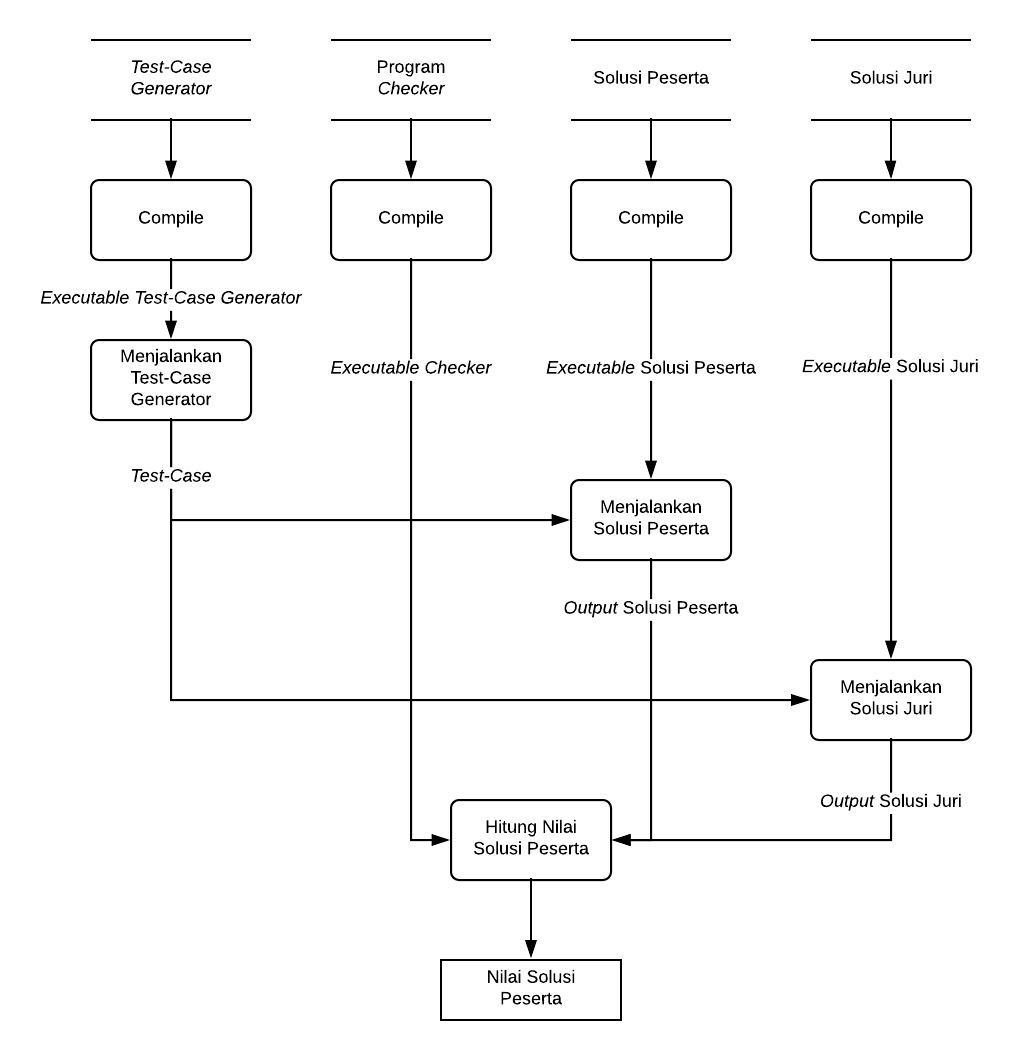
\includegraphics[width=0.85\textwidth]{images/grading-dfd}
    \caption{Diagram Aliran Data Pada Proses Penilaian Solusi Peserta}
    \label{fig:grading-dfd}
\end{figure}

\par Dengan menggunakan TCP dan TLS, kebocoran informasi yang dikirimkan melalui jaringan dapat dihindari sehingga tidak ada pihak ketiga yang dapat mengetahui isi dari informasi tersebut. Akan tetapi, karena informasi ini diterima oleh komputer peserta, peserta dapat dengan mudah mengetahui isi dari informasi tersebut. Oleh karena itu, diperlukan satu lapisan enkripsi lagi pada aplikasi yang berjalan pada komputer peserta.

\begin{figure}[ht!]
    \centering
    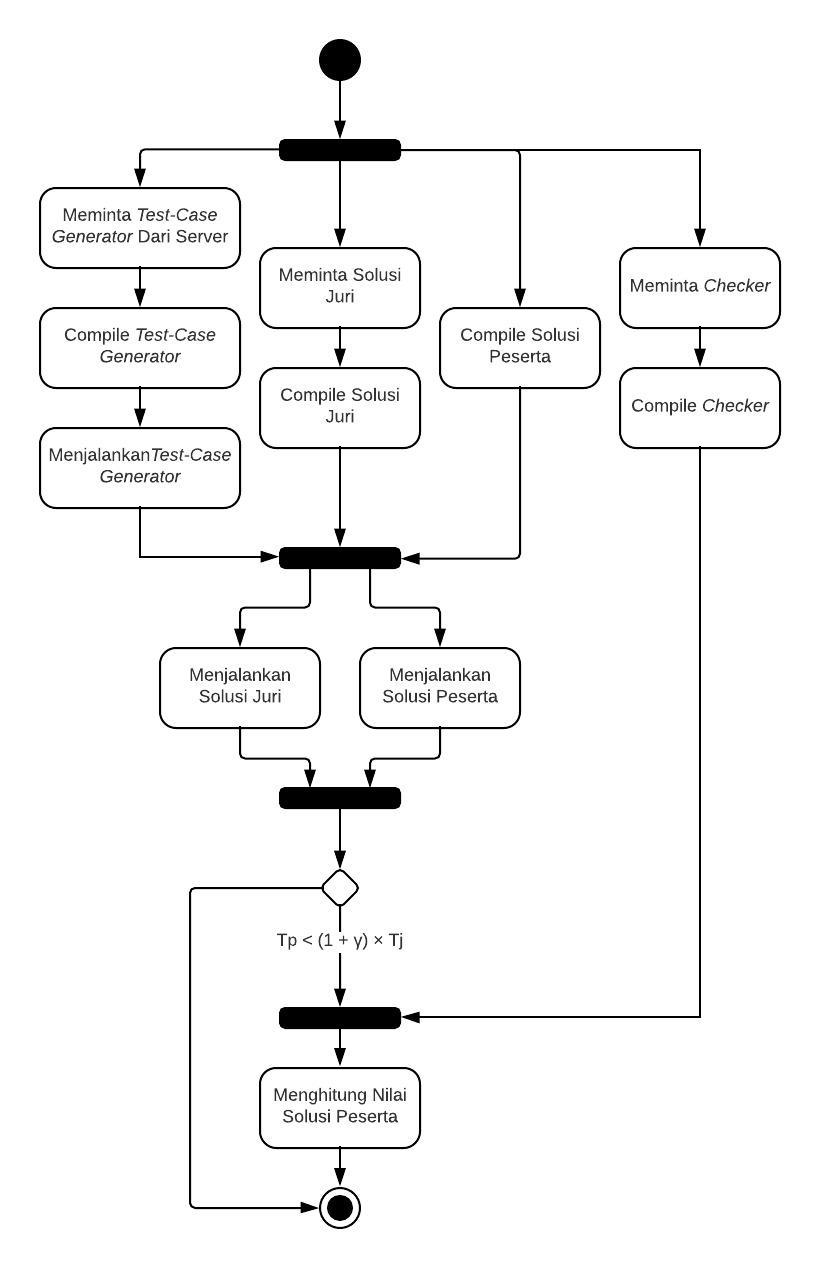
\includegraphics[width=0.65\textwidth]{images/total-grader-activity}
    \caption{Alur Proses Penilaian Jawaban Peserta}
    \label{fig:total-grader-activity}
\end{figure}

\par \textit{Test-case} umumnya merupakan file \textit{text} yang cukup besar. Pengiriman file ini dapat menghabiskan banyak \textit{bandwidth}. Meskipun begitu, \textit{test-case} biasanya dibuat dengan cara dibangkitkan oleh sebuah program yang dibuat oleh juri. \textit{Test-case} yang sama dapat dibangkitkan berulang-kali dengan menjalankan program tersebut. Untuk mengurangi kebutuhan \textit{bandwidth}, \textit{test-case} tidak perlu dikirim, melainkan program pembangkit \textit{test-case} saja yang dikirim. \textit{Test-case} yang akan digunakan untuk melakukan penilaian solusi peserta dibangkitkan dengan program pembangkit \textit{test-case} ini seperti pada Gambar \ref{fig:grading-dfd}. Diagram pada Gambar \ref{fig:total-grader-activity} menggambarkan alur proses penilaian jawaban peserta secara lengkap.

\par Pada tugas akhir ini, \textit{test-case} dipertukarkan dengan mengirimkan program pembangkit \textit{test-case} secara aman. Keamanan diperoleh dengan menggunakan dua kali enkripsi yaitu pada lapisan \textit{transport} dan aplikasi. Terdapat beberapa protokol yang dapat digunakan dalam melakukan pengiriman informasi ini. Protokol yang dipilih pada tugas akhir ini adalah protokol HTTP (\textit{hypertext transfer protocol}). Protokol ini dipilih karena aman dan mudah untuk digunakan.

\subsection{Menghadapi Serangan \textit{Reverse Engineering}}

\par Karena penilaian jawaban pada sistem \textit{online judge} yang dibangun dilakukan pada komputer peserta, maka muncul risiko adanya serangan \textit{reverse engineering} yang dapat dilakukan oleh pserta. Peserta dapat mengubah-ubah kode program dari \textit{autograder} yang dijalankan pada komputernya. Hal ini mengakibatkan peserta dapat mengubah kelakuan dari \textit{autograder}. Beberapa hal buruk yang mungkin terjadi antara lain adalah:
\begin{enumerate}
    \item Peserta dapat mengetahui kunci untuk melihat solusi juri dan \textit{testcase}.
    \item Peserta dapat selalu mengirimkan \textit{verdict} tertentu kepada sistem \textit{online judge}.
    \item Peserta dapat mengetahui jawaban dari peserta lain.
\end{enumerate}
Pada tugas akhir ini, diasumsikan peserta tidak melakukan serangan dalam bentuk \textit{reverse engineering}. Meskipun begitu, terdapat beberapa cara untuk mengurangi risiko yang muncul akibat serangan jenis ini.

\par Serangan \textit{reverse engineering} mungkin dilakukan oleh peserta jika peserta memiliki akses \textit{root} dari komputer yang digunakannya. Meskipun begitu, untuk beberapa jenis kompetisi \textit{competitive programming}, serangan ini dapat diatasi dengan tidak memberikan akses \textit{root} kepada peserta. Kompetisi ACM-ICPC merupakan salah satu jenis kompetisi yang dapat bertahan dari serangan \textit{reverse engineering}.

\par Pada kompetisi ACM-ICPC, peserta umumnya akan diseleksi terlebih dahulu secara bertingkat sebelum akhirnya berkompetisi di \textit{world final}. Sebelum babak \textit{world final}, jumlah peserta yang mengikuti kompetisi relatif sedikit sehingga sistem \textit{online judge} yang saat ini sering digunakan cukup untuk menjalankan kompetisi tersebut. Pada \textit{world final}, jumlah peserta kompetisi menjadi sangat banyak karena terdiri dari peserta-peserta yang lolos dari berbagai negara. Pada \textit{world final}, juri akan memberikan komputer khusus kepada peserta untuk mengikuti kompetisi tersebut. Pada babak \textit{world final}, juri dapat menggunakan komputer peserta sebagai \textit{worker} untuk menilai jawaban peserta. Juri dapat mengatur agar peserta tidak mendapatkan akses \textit{root} pada komputer yang digunakannya sehingga tidak dapat melakukan berbagai jenis serangan yang berupa \textit{reverse engineering}.

\par Untuk lebih mengurangi risiko yang muncul akibat serangan \textit{reverse engineering}, juri dapat mengatur agar setiap jawaban peserta dinilai oleh banyak \textit{worker}. Jika terdapat serangan \textit{reverse engineering} yang mengakibatkan \textit{worker} mengirimkan \textit{verdict} yang salah kepada \textit{server}, maka masih terdapat beberapa \textit{worker} lain yang mengirimkan \textit{verdict} yang benar. Peserta yang melakukan serangan \textit{reverse engineering} kemudian dapat dideteksi ketika \textit{verdict} yang dikirimkannya berbeda dengan peserta lain.

\par Sebagai contoh pada paragraf sebelumnya, misalkan setiap jawaban dinilai oleh lima buah \textit{worker}. Ketika sebuah jawaban dinilai, maka terdapat lima peserta berbeda yang melakukan penilaian. Seorang peserta bisa saja melakukan serangan \textit{reverse engineering} dan mengakibatkan \textit{worker} pada komputernya mengirimkan \textit{verdict} yang salah kepada \textit{server}. Meskipun begitu, empat peserta lain yang tidak melakukan serangan \textit{reverse engineering} akan mengirimkan \textit{verdict} yang berbeda dengan peserta yang melakukan serangan \textit{reverse engineering}. Dengan mengamati kelima buah \textit{verdict} ini, peserta yang mengirimkan \textit{verdict} yang berbeda dapat dikatakan melakukan serangan.

% TODO: tambah cara penilaian, pikirin lagi tentang self-grading, tambah penjelasan satu jawaban bisa dinilai lebih dari satu kali, jelasin grading_size

\section{Sistem Manajemen Kompetisi}

\begin{figure}[ht!]
    \centering
    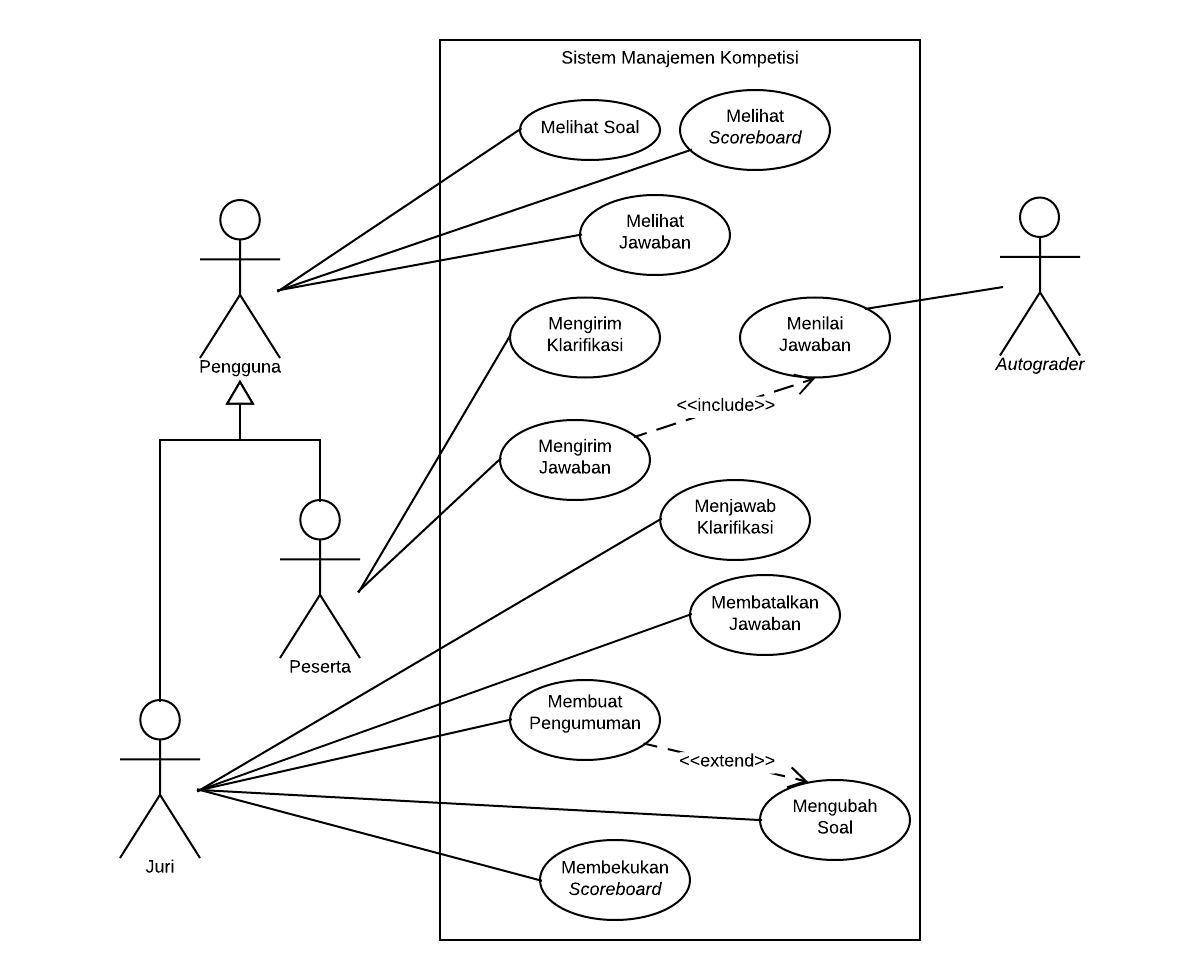
\includegraphics[width=0.85\textwidth]{images/oj-use-case}
    \caption{Diagram \textit{Use Case} Dari Sistem Manajemen Kompetisi}
    \label{fig:oj-use-case}
\end{figure}

\par Sistem manajemen kompetisi memberikan layanan kepada peserta kompetisi dan juri untuk berinteraksi. \textit{Online judge} yang populer pada saat ini memberikan sistem manajemen kompetisi berbasis \textit{web}. Sistem manajemen kompetisi ini dibutuhkan oleh peserta dan juri untuk melakukan aksi-aksi terkait kompetisi yang sedang berlangsung. Kebutuhan dari sistem manajemen kompetisi digambarkan oleh diagram \textit{use case} pada Gambar \ref{fig:oj-use-case}. Berikut ini adalah kebutuhan dari sistem manajemen kompetisi pada \textit{online judge}:

\begin{enumerate}
    \item Peserta dan juri dapat melihat soal.
    \item Peserta dapat mengirim jawaban.
    \item Sistem \textit{autograder} dapat menilai jawaban peserta.
    \item Peserta dapat mengirim klarifikasi soal.
    \item Juri dapat membuat pengumuman terkait kompetisi.
    \item Juri dapat menjawab klarifikasi peserta.
    \item Juri dapat mengubah soal.
    \item Peserta dan juri dapat melihat \textit{scoreboard}.
    \item Juri dapat membekukan \textit{scoreboard}.
    \item Peserta dapat melihat jawaban yang dikirim olehnya.
    \item Juri dapat melihat jawaban yang dikirim seluruh peserta.
    \item Juri dapat mengatur jawaban peserta untuk tidak dinilai.
\end{enumerate}

\par Pada tugas akhir ini, tidak semua kebutuhan dari sistem manajemen kompetisi diimplementasikan. Masalah yang ingin diselesaikan dalam tugas akhir ini tidak terletak pada sistem manajemen kompetisi, melainkan pada sistem \textit{autograder}. Oleh karena itu hanya kebutuhan yang berkaitan dengan proses penilaian saja yang diimplementasikan pada tugas akhir ini. Kebutuhan sistem manajemen kompetisi yang diimplementasikan pada tugas akhir ini antara lain adalah:

\begin{enumerate}
    \item Peserta dan juri dapat melihat soal.
    \item Peserta dapat mengirim jawaban.
    \item Sistem \textit{autograder} dapat menilai jawaban peserta.
    \item Juri dapat mengubah soal.
    \item Peserta dapat melihat jawaban yang dikirim olehnya.
    \item Juri dapat melihat jawaban yang dikirim seluruh peserta.
\end{enumerate}

\begin{figure}[ht!]
    \centering
    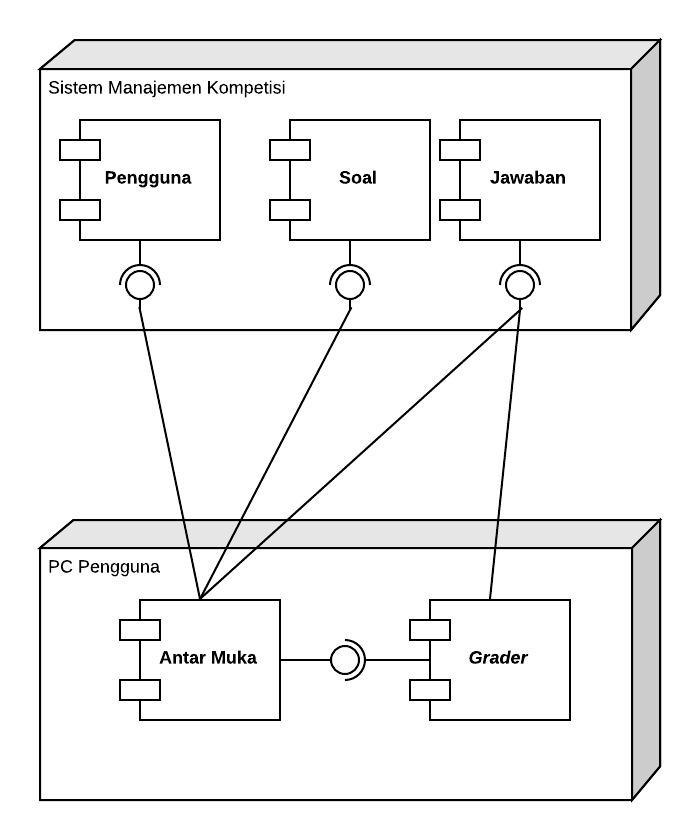
\includegraphics[width=0.5\textwidth]{images/oj-components}
    \caption{Diagram Komponen Sistem Manajemen Kompetisi}
    \label{fig:oj-components}
\end{figure}
% TODO: tambah komponen "kontes"

\par Sistem manajemen kompetisi yang digunakan pada tugas akhir ini mengikuti sistem manajemen kompetisi yang saat ini banyak digunakan. Sistem manajemen kompetisi ini dapat dibagi menjadi beberapa komponen utama yaitu: pengguna, soal, jawaban, antar muka dan \textit{grader}. Komponen \textit{grader} tidak lain adalah sistem \textit{autograder} yang telah dipaparkan pada bagian \ref{subsec:autograder}. Diagram komponen pada Gambar \ref{fig:oj-components} menggambarkan komponen yang digunakan dalam sistem manajemen kompetisi beserta keterhubungannya.

\subsection{Komponen Pengguna}

\par Kompetisi \textit{competitive programming} ada yang bersifat tertutup dimana hanya peserta tertentu yang dapat mengikutinya dan terbuka dimana setiap orang dapat mengikutinya. Sistem \textit{online judge} yang populer saat ini umumnya dapat menangani kedua jenis kompetisi tersebut. Untuk memasuki kompetisi, peserta perlu membuat akun di sistem \textit{online judge} tersebut terlebih dahulu. Peserta kemudian dapat memasuki kompetisi dengan cara melakukan \textit{login} pada sistem tersebut. Untuk menangani pendaftaran peserta baru dan \textit{login}, sistem \textit{online judge} perlu memiliki komponen manajemen pengguna yang bertugas melakukan otentikasi dan otorisasi pengguna. Beberapa \textit{online judge} memiliki komponen manajemen pengguna yang memanfaatkan layanan otentikasi dan otorisasi dari pihak ketiga seperti Google, Facebook, Github, dan Auth0. Terdapat juga sistem \textit{online judge} yang melakukan otentikasi dan otorisasi tanpa menggunakan pihak ketiga, misalnya DomJudge dan Mooshak.

\par Komponen pengguna dibuat pada sistem manajemen kompetisi untuk melakukan otentikasi dan otorisasi pengguna. Untuk menyederhanakan persoalan, pada tugas akhir ini komponen pengguna yang bertugas melakukan otentikasi dan otorisasi pengguna tidak akan menggunakan layanan pihak ketiga. Beberapa \textit{software development framework} seperti Django, Express, dan Laravel memiliki kemampuan untuk menangani masalah ini dengan mudah. Informasi pengguna akan disimpan pada sistem basis data yang sudah tersedia. Otentikasi pengguna akan dilakukan dengan sederhana, yaitu menggunakan \textit{username} dan \textit{password}.

\par Otorisasi pengguna juga dilakukan secara sederhana yaitu dengan sistem \textit{Role-based access control}. Setiap pengguna akan diberikan \textit{role} tertentu. Aksi-aksi yang dapat dilakukan oleh pengguna ditentukan oleh \textit{role} yang dimilikinya. Setiap pengguna yang berhasil \textit{login} kedalam sistem akan diberikan \textit{token} unik. \textit{Token} unik ini digunakan untuk menentukan \textit{role} dari pengguna yang melakukan aksi pada sistem. \textit{Token} yang akan digunakan dalam tugas akhir ini adalah JWT (JSON \textit{Web Token}) karena mudah untuk digunakan dan aman.

\subsection{Komponen Soal}

\par Pada kompetisi \textit{competitive programming}, deskripsi soal dapat diakses melalui sistem \textit{online judge} yang biasanya berupa halaman web. Dalam beberapa kompetisi, peserta kompetisi akan mendapatkan soal dalam bentuk \textit{hard-copy}. Komponen soal dibutuhkan oleh sistem manajemen kompetisi untuk mengelola soal yang ada pada kompetisi. Komponen ini memberikan layanan kepada pengguna untuk melihat soal. Terkadang terdapat kesalahan pada soal ketika kompetisi berlangsung sehingga komponen ini perlu memberikan layanan kepada juri untuk mengganti soal.

\par Soal pada kompetisi \textit{competitive programming} memiliki deskripsi yang merupakan penjelasan terhadap masalah yang harus diselesaikan peserta. Pada deskripsi soal terdapat penjelasan mengenai permasalahan yang dimaksud, format masukan, format keluaran, contoh masukan, dan contoh keluaran. \textit{Online judge} yang populer saat ini memberikan deskripsi soal kepada peserta dengan format \textit{pdf} atau menampilkannya dalam halaman web. Komponen soal perlu menyimpan deskripsi soal untuk dapat memberikannya kepada pengguna. Deskripsi soal dapat disimpan pada \textit{filesystem} dalam bentuk pdf atau disimpan dalam sistem manajemen basis data dalam bentuk HTML. Untuk memudahkan implementasi pada tugas akhir ini, deskripsi soal akan disimpan dalam basis data.

\par Setiap soal perlu memiliki program \textit{test-case generator}, \textit{solution}, dan \textit{checker}. Ketiga buah program ini dibuat oleh juri untuk melakukan penilaian jawaban peserta. \textit{Test-case generator} adalah program yang dibuat oleh juri untuk membangkitkan \textit{test-case} seperti yang sudah dijelaskan pada bagian \ref{subsec:sending-test-case-to-worker}. \textit{Solution} adalah program yang merupakan solusi valid dari soal. Program solusi ini dibuat oleh juri untuk dibandingkan dengan jawaban peserta seperti yang sudah dijelaskan pada bagian \ref{subsec:time-memory-measure-compare-with-jury}. Program \textit{checker} akan digunakan oleh \textit{worker} untuk menentukan kebenaran jawaban peserta. Terkadang terdapat lebih dari satu jawab yang benar pada sebuah soal. Oleh karena itu, program \textit{checker} ini dibutuhkan untuk menilai jawaban peserta. 

\par Program \textit{test-case generator}, \textit{solution}, dan \textit{checker} dapat disimpan dalam \textit{filesystem} atau sistem basis data. Pada tugas akhir ini, program-program tersebut disimpan pada \textit{filesystem} dan alamat dari program tersebut disimpan dalam sistem basis data.

\subsection{Komponen Jawaban}

\par Sistem manajemen kompetisi perlu menyediakan layanan kepada peserta untuk mengirimkan jawaban. Jawaban yang dikirimkan peserta berupa program dalam bentuk \textit{source code} dalam bahasa pemrograman yang diizinkan oleh juri. Selain itu, sistem manajemen kompetisi juga harus memberikan layanan kepada peserta untuk dapat melihat kembali jawabannya. Juri juga perlu mengawasi jawaban dari peserta untuk menghindari adanya kecurangan.  Oleh karena itu, sistem manajemen kompetisi juga harus dapat memberikan layanan kepada juri untuk melihat seluruh jawaban yang pernah dikirimkan oleh peserta. Pada sistem \textit{online judge} yang dibangun, komponen jawaban berguna untuk memberikan layanan-layanan tersebut. Pada tugas akhir ini jawaban peserta akan disimpan dalam bentuk \textit{file source code} pada \textit{filesystem}.

\subsection{Komponen Antar Muka}

\begin{figure}[ht!]
    \centering
    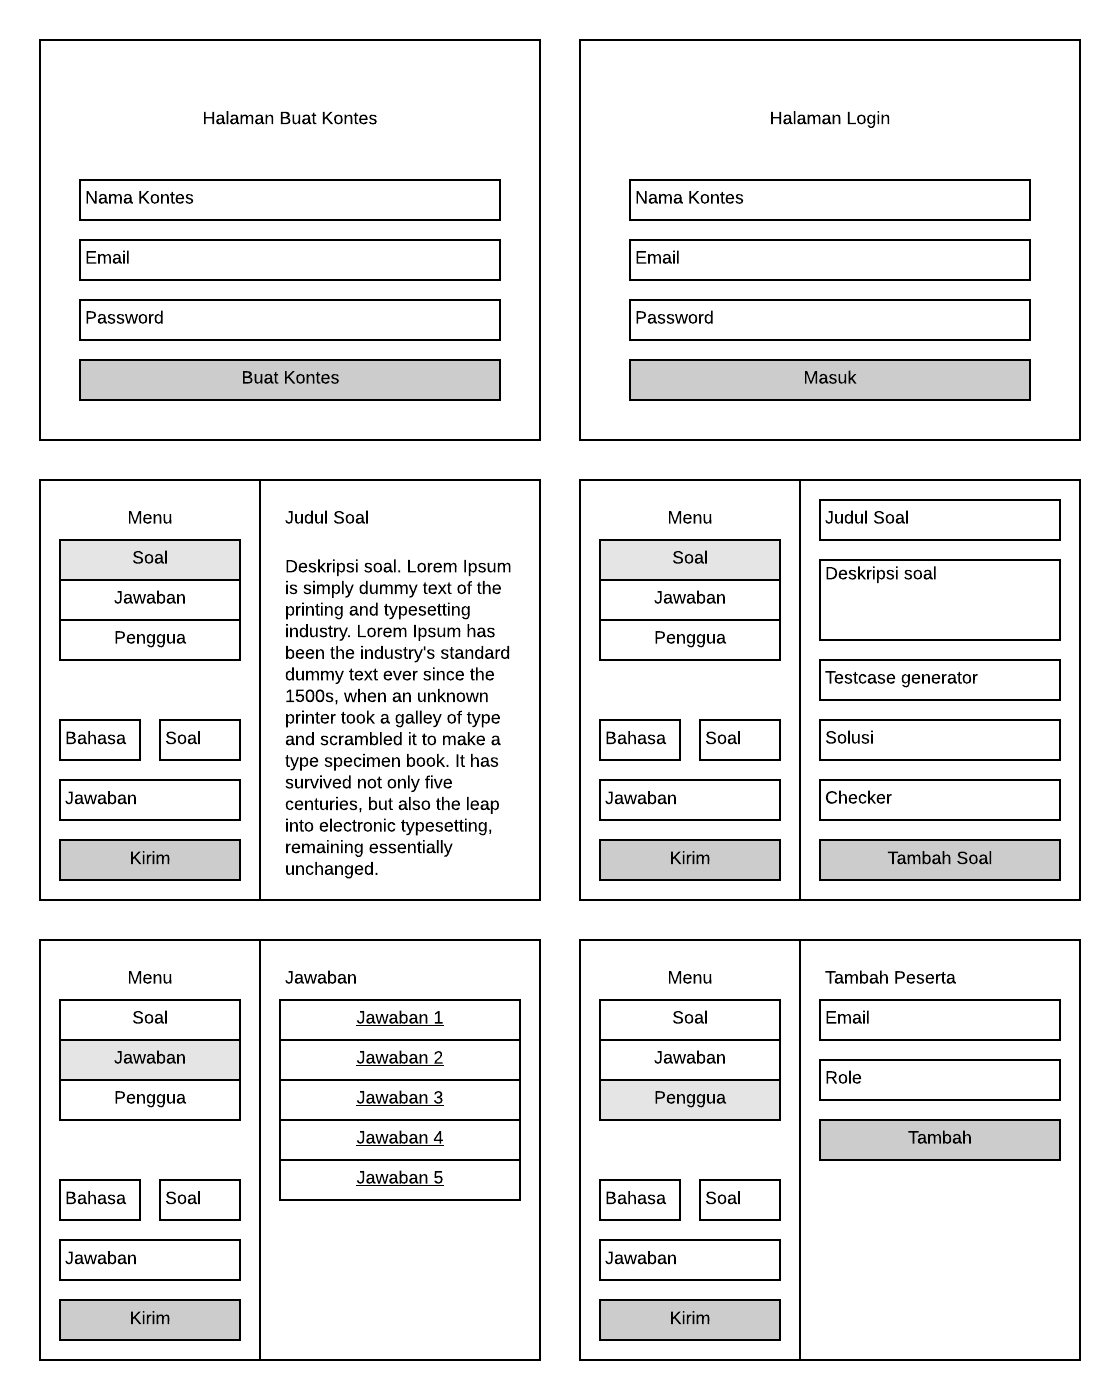
\includegraphics[width=0.85\textwidth]{images/mockup}
    \caption{Desain Tampilan Antar Muka Sistem \textit{Online Judge}.}
    \label{fig:mockup}
\end{figure}

\par Untuk memudahkan peserta dan juri berinteraksi dengan sistem \textit{online judge}, diperlukan komponen antar muka. Pengguna yang merupakan peserta dan juri menggunakan antar muka ini untuk melakukan aksi-aksi pada sistem \textit{online judge}. Kebanyakan sistem \textit{online judge} yang populer saat ini menggunakan antar muka berbasis \textit{web}. Antar muka berbasis \textit{web} digunakan karena mudah diakses oleh pengguna, dan cukup ringan untuk dijalankan.

\par Pada tugas akhir ini, antar muka dibuat dalam bentuk tampilan grafis berbasis web. Untuk memudahkan pengguna, antar muka dibuat sebagai aplikasi \textit{desktop}. Hal ini bertujuan agar komponen antar muka dan \textit{grader} dapat berjalan secara sekaligus. Gambar \ref{fig:mockup} merupakan rancangan halaman-halaman yang dibangun pada komponen antar muka.

% TODO: tambah penjelasan tentang submission, grading_group, grading, erd diagram dari db